\documentclass[11pt]{article}
\usepackage[utf8]{inputenc} 
%\usepackage[latin1]{inputenc}
\usepackage[T1]{fontenc}
\usepackage[french]{babel}
\usepackage{lmodern}


%\usepackage{setspace}
\usepackage[bottom=3cm, top=3cm,left=4cm, right=4cm]{geometry}

\usepackage{float}
\usepackage{graphicx}
%\usepackage{wrapfig}
\usepackage{epstopdf}

\usepackage{amsthm}
\usepackage{amsmath}
\usepackage{amssymb}
\usepackage{mathrsfs}

%\usepackage[overload]{empheq}


\newtheorem{champ_parallele}{Définition}
\newtheorem{geodesique}{Définition}
\newtheorem{unicite}{Lemme}
\newtheorem{isometrie}{Définition}

\pagestyle{headings}

\makeatletter
\def\clap#1{\hbox to 0pt{\hss #1\hss}}%
\def\ligne#1{%
\hbox to \hsize{%
\vbox{\centering #1}}}%
\def\haut#1#2#3{%
\hbox to \hsize{%
\rlap{\vtop{\raggedright #1}}%
\hss
\clap{\vtop{\centering #2}}%
\hss
\llap{\vtop{\raggedleft #3}}}}%
\def\bas#1#2#3{%
\hbox to \hsize{%
\rlap{\vbox{\raggedright #1}}%
\hss
\clap{\vbox{\centering #2}}%
\hss
\llap{\vbox{\raggedleft #3}}}}%
\def\maketitle{%
\thispagestyle{empty}\vbox to \vsize{%
\haut{}{\@blurb}{}
\vfill
\vspace{1cm}
\begin{flushleft}
\usefont{OT1}{ptm}{m}{n}
\huge \@title
\end{flushleft}
\par
\hrule height 4pt
\par
\begin{flushright}
\usefont{OT1}{phv}{m}{n}
\Large \@author
\par
\end{flushright}
\vspace{1cm}
\vfill
\vfill
\bas{}{\@location, \@date}{}
}%
\cleardoublepage
}
\def\date#1{\def\@date{#1}}
\def\author#1{\def\@author{#1}}
\def\title#1{\def\@title{#1}}
\def\location#1{\def\@location{#1}}
\def\blurb#1{\def\@blurb{#1}}

\blurb{}
\makeatother

\title{Calorimétrie et boson de Higgs}
\author{ Maëlle Joveneau \\ Manuel Tondeur \\ Brieuc François }
\date{Année académique 2011-2012}
\location{Louvain - La - Neuve}

\blurb{%
Université Catholique de Louvain\\
Faculté des Sciences\\
\textbf{LPHY2135-Computing et Méthodes numériques en physique des particules}\\
Bruno Giacomo Luca}% 

\setlength{\parskip}{1ex plus .6ex minus .6ex}
\renewcommand\arraystretch{1.5}
%\onehalfspacing

\begin{document}

	\maketitle
		
	\tableofcontents

	\newpage
	
			\section{Introduction}
	Afin de d\'ecouvrir les principes de bases de Geant4, un framework conçu
pour la physique des particules, nous avons cr\'eé un programme permettant de
d\'eterminer la masse du Higgs en simulant la d\'esint\'egration de celui-ci en
deux $Z^0$ qui eux-m\^emes se d\'esint\`egrent en $e^-$ $e^+$.

Pour ce faire nous avons d'abord dû construire un d\'etecteur qui soit efficace
pour notre d\'esint\'egration. Nous avons d\'etermin\'e que les \'el\'ements
n\'ecessaires pour ce d\'etecteur \'etaient : des calorim\`etres
\'electromagn\'etiques et des trackers. Nous avons donc dû utiliser les classes
de Geant4 adaptées à nos besoins.
 
Nous avons alors g\'en\'er\'e nous-m\^eme les diff\'erentes particules qui
apparaissent dans l'\'ev\`enement qui nous int\'eresse. Pour donner aux
diff\'erentes particules leur masse, leur \'energie, et/ou leur impulsion, nous
avons dû faire appel \`a des fonctions de distribution vari\'ees qui nous ont
permises de mettre en pratique la th\'eorie des variables aléatoires dont la
méthode "Monte Carlo".
 
A partir des classes abstraites de Geant4, nous avons défini les interactions
possibles entre les particules et les \'el\'ements pr\'esents au sein du
d\'etecteur. Cela fait, il nous fallait reconstruire la trajectoire des
\'electrons \`a partir des informations fournies par les trackers et les
calorim\`etres. Avec celles-ci, nous avons pu d\'eterminer l'\'energie et
l'impulsion des quatre \'electrons qui nous donnent la masse du Higgs par la
relation de la masse invariante suivante : 
 
\begin{equation}
M_H^2=E_H^2-p_H^2=(E_1+E_2+E_3+E_4)^2-(\vec{p}_1+\vec{p}_2+\vec{p}_3+\vec{p}_4)^2.
\end{equation} 
    
Les erreurs dues aux bruits ont \'et\'e introduites dans la simulation, ce qui
nous poussa à posé un seuil d'\'energie au niveau de la 
d\'etection. Pour inclure les erreurs syst\'ematiques, 4 électrons d'énergie connue ont été lancés 1200 fois dans 
le détecteur. Les diff\'erences entre l'énergie détectée et l'énergie vraie sont alors mesurées et pondérées avec 
l'énergie vraie. Le facteur correctif est déterminé en conséquence. Les
d\'etails de toutes ces \'etapes sont pr\'esent\'es dans la suite de ce rapport.





		    \section{Descriptifs des méthodes et résultats}

\subsection{Description du détecteur}

Pour la construction du détecteur nous avons opté pour une géométrie cylindrique
de type CMS que nous avons bien entendu simplifiée pour ne garder que les
éléments utiles à notre simulation. Le détecteur est donc constitué de plusieurs
trackers en forme de tubes imbriqués et d'un calorimètre
électromagnétique granulaire qui englobe le tout. Ces éléments sont placés dans
le "world volume" que nous avons choisi de remplir d'air pour se rapprocher de
la réalité.

Comme dans le CMS, les trackers sont faits de silicium et mesurent 27.2 m de
long. Ils sont au nombre de treize, nous en avons mis trois très proches du
centre, le premier étant à 8 cm du vertex et les deux autres espacés de 1 cm du
premier. Les dix autres trackers se trouvent espacés chacun de 10 cm, le premier
ayant un rayon 20 cm. Bien qu'il nous faille plusieurs trackers pour obtenir
une bonne résolution sur la direction des particules, ce choix particulier est
simplement
fait pour se rapprocher du CMS. Étant donné que notre projet ne nécessite
aucunement un champ magnétique, nous avons simplement choisi de ne pas en
mettre pour ne pas nous compliquer la tâche inutilement. 

Le bloc de calorimètres est un gros tube de 28 m de long dont
l'épaisseur s'étend de 1.5 m du centre à 3 m du centre. Il est uniquement
composé de calorimètres électromagnétiques car l'événement d'intérêt n'implique
ni muon ni hadron. L'épaisseur fût choisie pour éviter toute perte d'énergie.

Les cellules, composées d'Iodure de Cesium, sont relativement grosses par
rapport à celles du CMS. En effet, les événements considérés au CMS impliquent
un grand nombre de particules qu'il faut pouvoir distinguer les unes des
autres. Notre simulation n'ayant que quatre particules identiques à considérer,
nous pouvons tout à fait nous permettre cette simplification. La taille des
cellules fut donc choisie pour correspondre à la taille d'un jet de sorte que
l'énergie d'un jet se dépose presque toujours dans maximum quatre d'entre elles.

NB : on trouvera les détails de la construction des détecteurs dans les classes
suivantes : \textit{"projetZTrackerParametrisation.cc",
"projetZCaloParametrisation.cc", "projetZTrackerSD.cc", "projetZCaloSD.cc"} et 
\textit{"projetZDetectroConstruction.cc"}. 



\subsection{Description physique du processus initial}

Pour rappel, le but de ce projet est de reconstruire la masse invariante du
boson de Higgs à l'aide de la détection de l'énergie de quatre électrons issus
du processus suivant :

\begin{equation}
H \longrightarrow ZZ \longrightarrow e^+ e^- e^+ e^-.
\end{equation}

Voyons maintenant en détail la méthodologie utilisée dans ce but. Dans un
soucis de réalisme, nous avons choisi de ne pas fixer la masse du $H$ mais
de la générer aléatoirement avec une distribution de Breit-Wigner centrée sur
200 GeV et de demi largeur 2.5 GeV. Nous avons dans un premier temps étudié la reconstruction de sa masse
invariante lorsque le Higgs se désintègre au repos pour ensuite se rapprocher
de la réalité en considérant sa désintégration alors qu'il est en mouvement dans
le repère du détecteur. Dans ce but, nous générons une énergie cinétique issue
d'une distribution exponentielle négative de paramètre 30 GeV ainsi que deux
angles $\theta$ et $\varphi$ issus de distributions uniformes pour lui donner
une direction\footnote{On trouvera les différentes distributions dans la classe
"\textit{projetZDistribution.cc}".}. La distribution uniforme des angles se
justifie par le fait que le mécanisme dominant de création du $H$ est $ g g
\to H$ qui ne donne aucun dépendance angulaire. 

Nous nous plaçons
ensuite dans le repère où il est au repos pour simuler sa désintégration en deux
bosons $Z$. La cinématique relativiste du processus est assez simple et tous les
paramètres sont fixés hormis la direction d'émission (nous avons choisi de
négliger le caractère aléatoire de la masse du Z qui est dû à l'incertitude
d'Heisenberg $\Delta E \Delta t \geq \hbar$ car cela est sans intérêt pour notre
discussion). Pour la direction, nous générons à nouveau deux angles de manière
uniforme mais la justification vient cette fois de l'absence de spin du $H$. 

La même méthode est appliquée pour simuler la désintégration des $Z$ en
$e^+e^-$ Nous avons donc quatre électrons d'énergie et de direction bien
déterminées dans le repère de leur parent $Z$ respectif. Il suffit alors
d'effectuer les boosts de Lorentz adéquats pour retourner dans le repère du $H$
et ensuite dans le repère du détecteur\footnote{Toutes ces manipulations pour
simuler la désintégration du Higgs sont des algorithmes ne nécessitant pas le
framework "Geant4".}. On trouvera les détails de ces manipulations dans la
classe "\textit{projetZElectronsGenerator.cc}".

NB: les temps de vie très court
du $H$ et du $Z$ nous permettent en très bonne approximation de considérer que
les quatre électrons sont émis au centre géométrique de notre détecteur. 

L'étape
suivante consiste à "lancer" ces quatre électrons dans notre détecteur à l'aide
du framework Geant4. Cela est implémenté dans la classe
"\textit{projetZPrimaryGeneratorAction.cc}".

Le choix des interactions discrètes autorisées pour chacune des particules est
assez simple puisque nous n'avons en jeux que des électrons-positrons et des
photons cf "\textit{projetZPhysicsList.cc}". Le voici tout de même : 
\begin{itemize}
\item photons : création de paires électrons-positrons, diffusion Compton et
effet photoélectrique.
\item électrons : ionisation, bremsstrahlung et diffusion multiple.
\item positrons : ionisation, bremsstrahlung, diffusion multiple et
annihilation avec un électron.\\ 
\end{itemize}

A titre informatif, on peut voir sur les figures ci-dessous l'illustration de
deux Higgs différents qui se désintègrent dans le détecteur.
La figure (\ref{viz1}) montre clairement les quatre jets séparément (nous avons
choisi de ne montrer que les particules de plus de 100 MeV pour la propreté). La
figure (\ref{viz2}) montre toutes les particules de plus de 20 MeV. Cette
dernière fait apparaître la structure des trackers ainsi que l'importance des
particules secondaires qui "rebondissent" un peu partout et génèrent ainsi
des hits indésirables dans nos trackers.

\begin{figure}
\caption{Visualisation d'un événement ne montrant que les particules de plus
de 100 MeV}
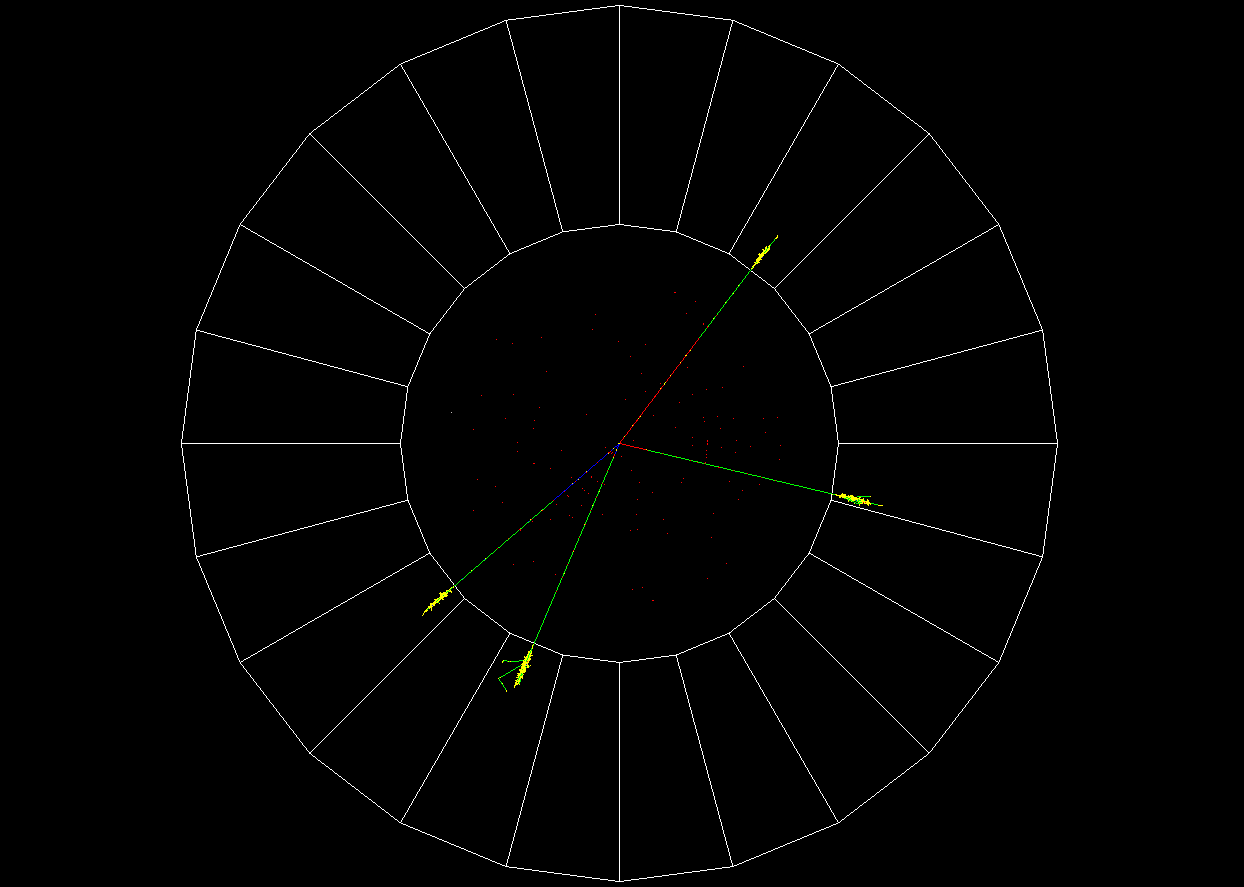
\includegraphics[scale=0.40]{images/evenPlus100MeV.png}
\label{viz1}
\end{figure}

\begin{figure}
\caption{Visualisation d'un événement ne montrant que les particules de plus
de 20 MeV}
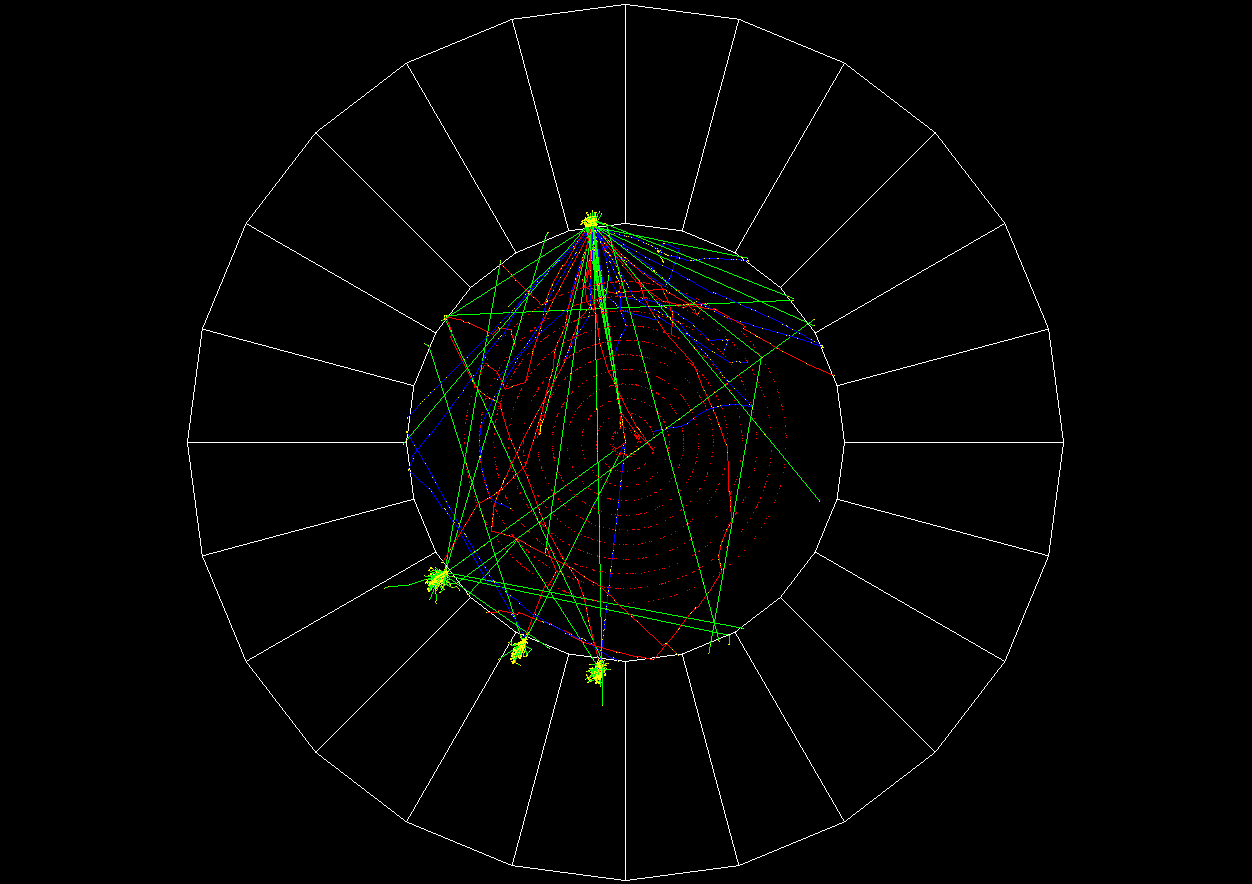
\includegraphics[scale=0.40]{images/evenPlus20MeV3.png}
\label{viz2}
\end{figure}

\newpage
\subsection{Reconstruction de la masse invariante du boson de Higgs}

Une fois les électrons lancés dans le détecteur, nous obtenons une réponse sous
forme d'un ensemble de "hits" aussi bien pour le tracker que pour le
calorimètre. Les détails de l'implémentation des hits se trouvent dans les
classes "\textit{projetZTrackerHit.cc}" et "\textit{projetZCaloHit.cc}".
L'information
d'intérêt dépend de la pièce du détecteur qui renvoit les donnnées du  hit eg
pour les trackers, seule la position du hit nous intéresse tandis que pour le
calorimètre c'est l'énergie déposée qui est utile.

Présentons les choses dans l'ordre d'utilisation de notre code. Chaque cellule
du calorimètre nous renvoie l'énergie totale déposée en elle par
l'intermédiaire d'une liste de hits. Grâce à un
algorithme de cluster qui sera explicité plus loin, nous pouvons isoler de
cela quatre jets distincts (dans la majorité des cas) et extraire de ces
informations l'énergie totale et l'endroit ou chacun des électrons s'est
arrêté. L'énergie déposée dans les trackers et dans l'air est en effet
insignifiante par rapport aux énergies en jeux. Comme la trajectoire des
particules dans le détecteur est rectiligne, la position des différents jets
dans le calorimètre nous donne immédiatement une information précieuse sur la
direction de l'impulsion initiale des électrons aux
vertex. Cependant, nos cellules ayant une relativement grande taille, la
précision sur cette direction est assez médiocre... C'est pourquoi nous avons
choisi d'affiner cette information à l'aide des trackers. Avoir une idée de la
direction des impulsions grâce aux cellules du calorimètre simplifie
grandement l'algorithme utilisé pour obtenir cette direction plus précisément à
l'aide des trackers. En effet, nous avons considéré un cône d'ouverture
40$^{\circ}$
(valeur affinées par essais-erreurs) dont la pointe est le vertex et dont l'axe
relie ce dernier à la position centrale du jets. La "vraie" direction de
l'impulsion initiale de l'électron est obtenue en faisant une moyenne de toutes
les directions données par les trackers en ne tenant compte que des hits à
l'intérieur de ce cône. NB: l'utilisation du cône est nécessaire car le
tracker
nous donne les hits de tous les électrons y compris ceux qui rebondissent sur
le calorimètre et reviennent dans le tracker. 

Pour l'algorithme de cluster, nous avons opté pour une solution assez directe :
l'algorithme parcourt chacune des cellules et compare l'énergie
détectée dans cette cellule avec celles détectées dans les cellules voisines.
Si la cellule en question est celle qui possède le maximum, nous la retenons.
L'énergie totale du jet est obtenue en y ajoutant les trois énergies
maximales voisines. Pour que cet algorithme soit efficace, il faut bien entendu
supprimer toutes les cellules ayant reçu un peu d'énergie suite à
l'introduction du bruit. Après
plusieurs essais, nous avons choisi de fixer le seuil à 6 GeV pour éviter de
compter parfois 5 jets au lieu de quatre à cause du bruit ( le bruit est tiré
aléatoirement d'une gaussienne centrée sur 0 et de largeur 1 GeV et il arrivait
que des énergies fantômes montent jusqu'à 5 GeV à cause de l'effet combiné du
bruit et de particules parasites). Bien sûr, cette énergie seuil
donne lieu à des erreurs systématiques lorsque le jet est réparti par exemple
sur trois cellules et que la quatrième ne reçoit que quelques GeV. Cette
énergie est donc éliminée par le seuil, mais ce problème peut-être en partie
solutionné. En effet, une fois calibré, la perte moyenne d'énergie due à ce
phénomène est corrigée si nous prenons nos données sur un suffisamment grand
nombre d'événements. Le seul effet négatif est l'élargissement de la gaussienne
centrée sur la "vraie" valeur de la masse du Higgs.

NB: l'algorithme du cluster et de la reconstruction de la direction des
impulsions au vertex peut-être trouvé dans "\textit{projetZRunManager.cc}"

Cet algorithme possède un autre défaut, lorsque deux jets sont l'un à coté de
l'autre, l'énergie de certaines cases provient des deux jets et notre
algorithme la comptera donc deux fois. A titre d'exemple visuel, voici quelques
graphiques illustrant les différents cas rencontrés. Sur la figure (\ref{bonb})
on voit un événement avec bruit correspondant aux cas où notre algorithme
fonctionne parfaitement. Le même cas après introduction du seuil d'énergie est
illustré sur la figure (\ref{bonp}). Ensuite viennent les cas où nous
rencontrons le problème du surcomptage de l'énergie sur les cases "partagées"
(voir figure (\ref{pasbonb}) et (\ref{pasbonp})).

\begin{figure}[p]
\caption{Résultat typique d'une détection de 4 jets parfaits par le cluster avec
bruit}
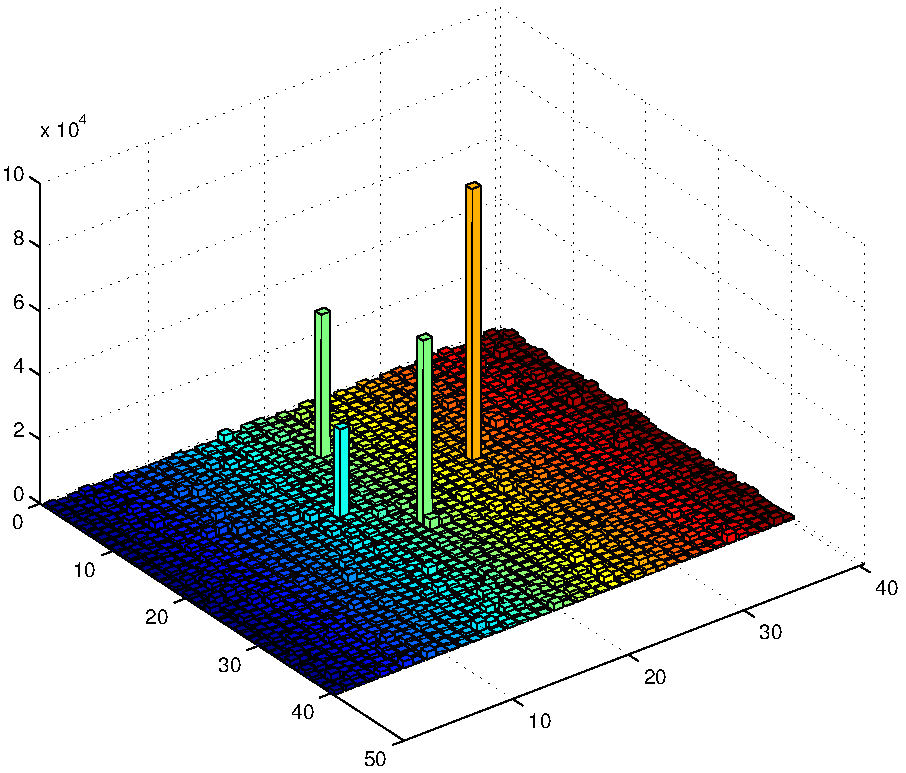
\includegraphics[scale=0.55]{images/bonCasBrut-eps-converted-to.pdf}
\label{bonb}
\end{figure}
\begin{figure}[p]
\caption{Résultat typique d'une détection de 4 jets parfaits par le cluster
après nettoyage du bruit}
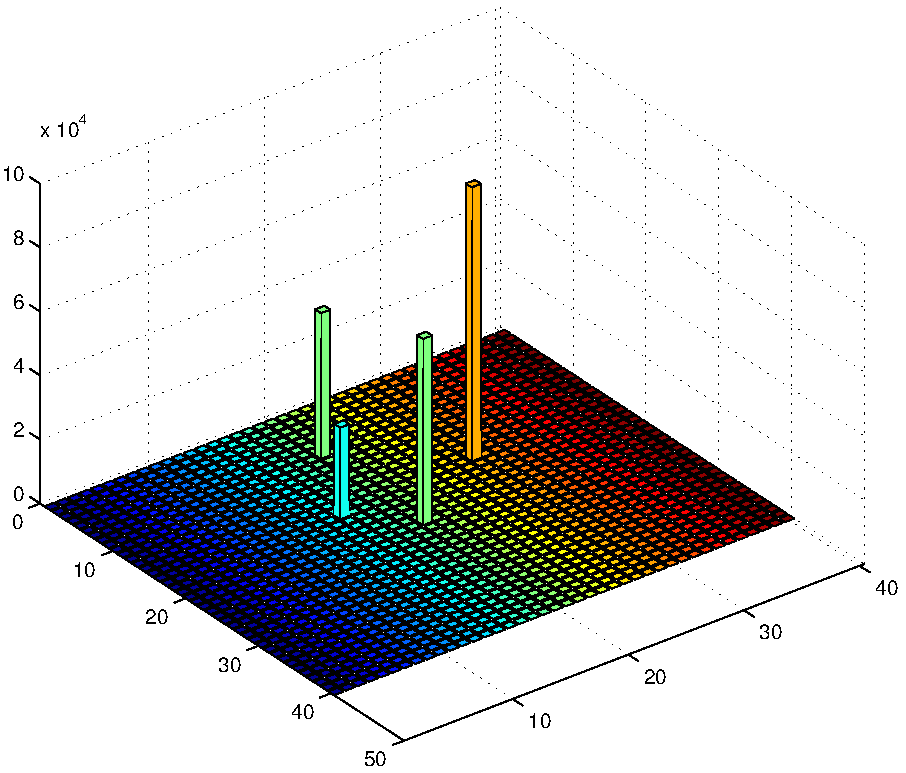
\includegraphics[scale=0.55]{images/bonCasNet-eps-converted-to.pdf}
\label{bonp}
\end{figure}
\begin{figure}[p]
\caption{Résultat d'une détection dite à problème.\newline On peut voir au
niveau des deux jets les plus à gauche le problème du double comptage d'énergie}
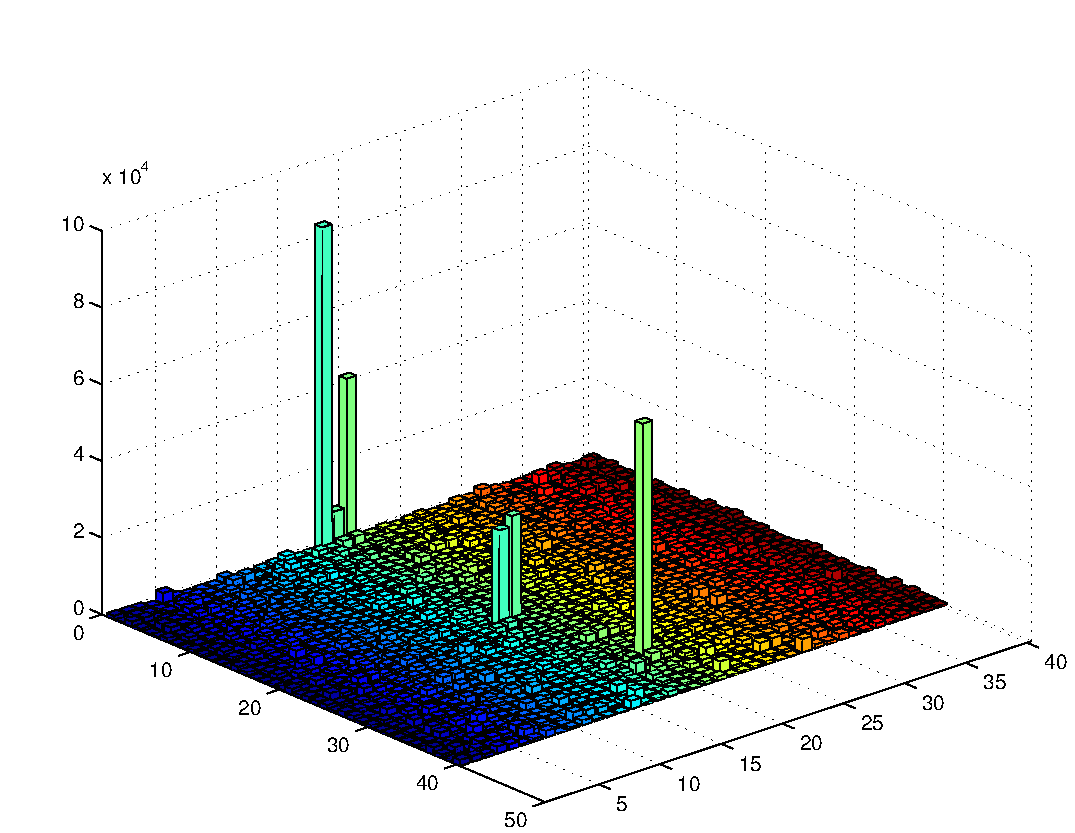
\includegraphics[scale=0.55]{images/mauvaisCasBrut-eps-converted-to.pdf}
\label{pasbonb}
\end{figure}
\begin{figure}[p]
\caption{Même après nettoyage du bruit, le problème reste présent}
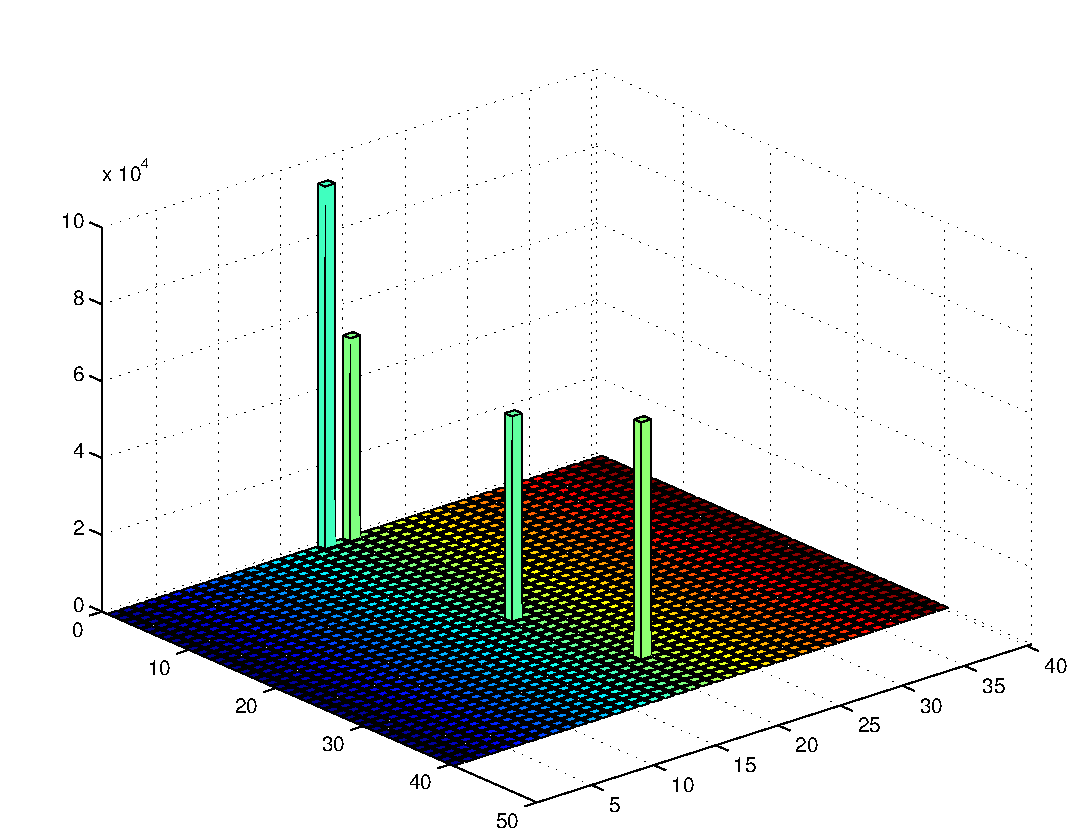
\includegraphics[scale=0.55]{images/mauvaisCasNet-eps-converted-to.pdf}
\label{pasbonp}
\end{figure}

\newpage
\subsection{Analyse des résultats}

Une fois tout cela implémenté, nous avons fait tourner le programme en boucle
1500 fois pour mesurer un grand nombre de masses du Higgs. C'est avec grand
plaisir que nous constatons que la distribution obtenue est fort proche de celle
attendue. Il suffit de regarder les figures (\ref{bw}) et (\ref{hist}) pour voir
que, bien que l'algorithme ne soit pas parfait, les résultats sont plus
qu'acceptables. Nous obtenons en effet une moyenne de 199.8950 GeV (rappel : le
centre de la Breit-Wigner de la masse du Higgs est à 200 GeV) pour un
écart type de 7.0826 GeV. Sur les 1500 Higgs créés, 1356 ont générés des
événements que notre algorithme à pu identifier correctement et reconstruire.
Cela fait moins de 10\% de pertes. Une première remarque sur l'histogramme des
résultats est que le nombre maximum d'événements se trouve un peu au dessus du
200 GeV mais cela serait explicable par une fluctuation statistique. Une seconde
remarque est l'apparition d'événements fort éloignés de 200 GeV. Cela pourrait
être dû aux failles de nos algorithmes ou bien également à une fluctuation
statistique mais quoi qu'il en soit, cela ne concerne que quelques événements
sur 1356 et est donc négligeable.

\begin{figure}[p]
\caption{Distribution Breit-Wigner des masses des Higgs générés}
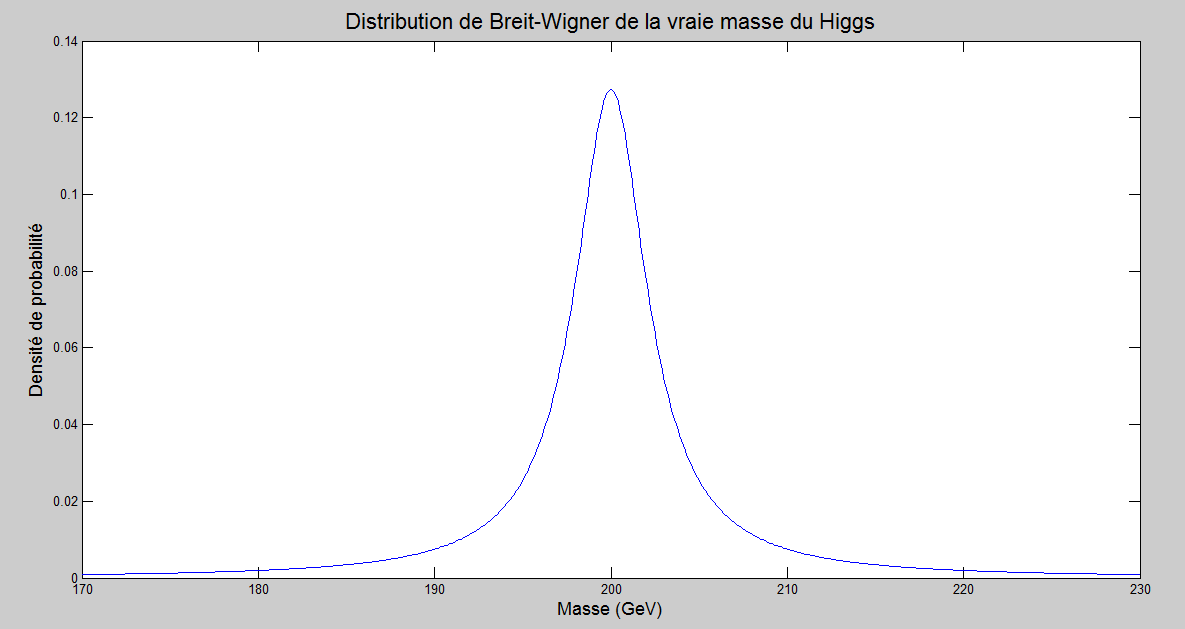
\includegraphics[scale=0.4]{images/bwmH.png}
\label{bw}
\end{figure}

\begin{figure}[p]
\caption{Histogramme des masses mesurées par notre détecteur}
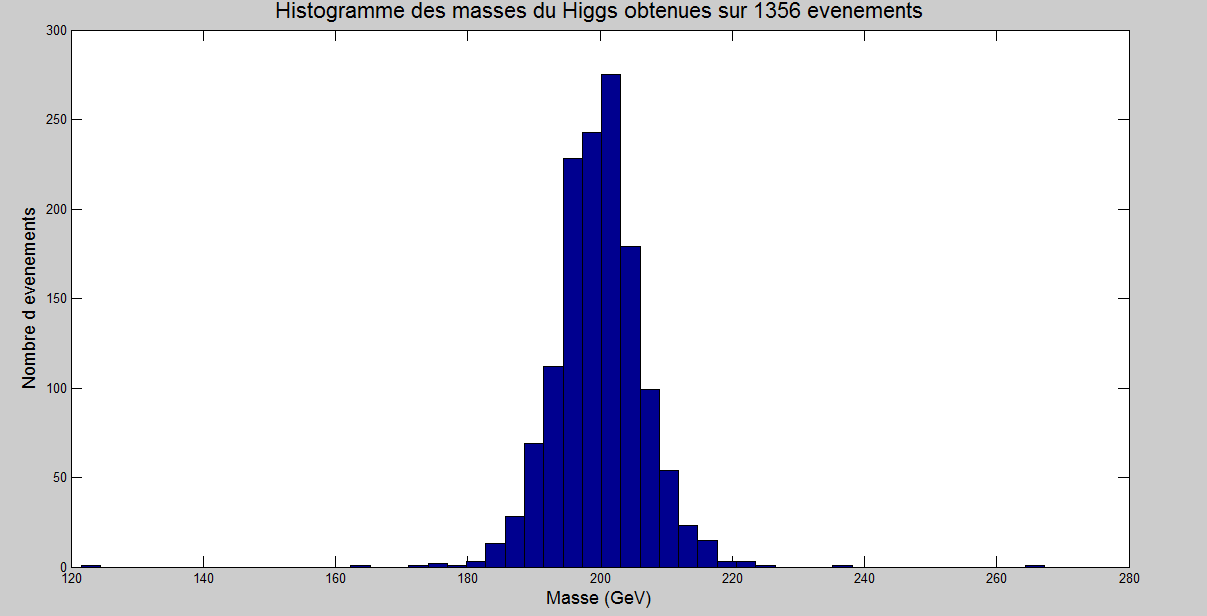
\includegraphics[scale=0.4]{images/histmH.png}
\label{hist}
\end{figure}


\newpage
\newpage
\section{Conclusion}
 Il apparait clairement dans la section pr\'ec\'edente que nous avons r\'eussi \`a obtenir la masse du Higgs.
Cependant, notre programme n'est pas optimal, il serait possible de le rendre plus rapide et 
moins couteux en m\'emoire vive. La pr\'ecision pourrait \'egalement être augment\'ee. 

Une première amélioration serait de refermer le d\'etecteur c'est-à-dire de placer des d\'etecteurs aux extrémités, 
perpendiculairement à l'axe des z dans notre cas (en laissant évidemment un
espace libre pour permettre le passage des 
particules dans le d\'etecteur). 

Au niveau de l'algorithme du cluster, on remarque que si deux jets sont très proches l'un de l'autre (une seule case 
s\'eparant deux maxima d'énergie détectés) alors l'énergie se trouvant sur cette
case est comptée deux fois. Cet algorithme
 pourrait être modifié de sorte que la quantité soit partagée équitablement
entre les deux jets.

Une autre façon de limiter le surcomptage de l'énergie, serait de raffiner les 
cellules. En effet, cela diminuerait la probabilité de "case" partagée et même dans les cas où cela se produirait, la
quantité d'énergie partagée serait moindre. Cependant cela nécessiterait une modification de notre 
algorithme 
étant donné qu'il est basé sur le fait qu'un jet ne puisse pas occuper
plus de quatre cellules.

Une dernière suggestion d'amélioration concernant l'algorithme de cluster serait
de limiter le nombre
de Higgs "perdus". En effet, dans le cas présent, nous jetons tous les
événements où nous ne détectons pas exactement quatre jets. Seul un algorithme
plus complexe pourrait nous permettre d'exploiter certains de ces cas
particuliers. Les Higgs étant ici simulés informatiquement, ils ne nous coûtent
pas très cher.

L'algorithme de reconstruction de la trace est assez basique et par conséquent
pas des plus précis. Il aurait sans doute
été préférable d'utiliser un algorithme plus complexe du type régression linéaire.


Certaines de ces améliorations auraient nécessité beaucoup de temps 
pour parfois peu d'amélioration au niveau de la précision. Nous avons tenté de
faire au plus proche de la réalité en passant du temps sur les points qui nous
semblaient prioritaires. Nous avons cherché le juste milieu entre l'amélioration
des résultats obtenus et le temps nécessaire pour y parvenir tout en ne
négligeant
pas nos autres cours et autres obligations.


		
\end{document}










			